% ============================================================
%  Beamer 演示：LLM 部署研究与资源安排
%  XeLaTeX + xeCJK 中文支持
%  源文档：notes.tex
% ============================================================
\documentclass[UTF8,11pt,aspectratio=169]{beamer}
\usepackage{xeCJK}
\setCJKmainfont{Songti SC}
\setCJKsansfont{Heiti SC}
\setCJKmonofont{STFangsong}

% ---------- 主题 ----------
\usetheme{Madrid}
\usecolortheme{whale}
\usefonttheme{professionalfonts}

% ---------- 包 ----------
\usepackage{graphicx}
\usepackage{booktabs}
\usepackage{amsmath,amssymb}
\usepackage{multirow}
\usepackage[table]{xcolor}
\usepackage{tikz}
\usepackage{hyperref}

% ---------- 信息 ----------
\title[LLM 部署研究]{LLM 部署研究与资源安排}
\subtitle{IC 设计 内网部署研究}
\author{葛良晨 by DeepSeek }
\date{2026-05-17}
\institute{数字IC}

% ---------- 自定义颜色 ----------
\definecolor{darkgreen}{RGB}{0,128,0}
\definecolor{darkred}{RGB}{180,0,0}
\definecolor{gold}{RGB}{200,150,0}

% ---------- 自定义 block 环境 ----------
\newenvironment{keypoint}{
  \begin{block}{\textbf{关键结论}}
}{
  \end{block}
}

\newenvironment{warningblock}{
  \begin{alertblock}{\textbf{⚠ 注意}}
}{
  \end{alertblock}
}

% ---------- 精简目录 ----------
\AtBeginSection[]{
  \begin{frame}{目录}
    \tableofcontents[currentsection]
  \end{frame}
}

\begin{document}

% ============================================================
%  标题页
% ============================================================
\begin{frame}
  \titlepage
\end{frame}

% ============================================================
%  目录
% ============================================================
\begin{frame}{目录}
  \tableofcontents[hideallsubsections]
\end{frame}

% ============================================================
%  第一章：LLM 本地部署的底层原理
% ============================================================
\section{LLM 本地部署的底层原理}

\begin{frame}{为什么先讲原理？}
  \begin{alertblock}{常见误区}
    看别人说「RTX 4090 能跑 70B 模型」就行——\textbf{能跑 $\neq$ 能用}，这之间差了一整个工程体系。
  \end{alertblock}

  \vspace{0.5em}
  必须理解：
  \begin{itemize}
    \item 显存到底存了什么？
    \item 为什么 Prompt 越长越慢？
    \item 量化到底压缩了什么？
    \item CPU/GPU 推理的真正瓶颈在哪？
  \end{itemize}
\end{frame}

% -------------------- 1.1 推理系统组成 --------------------
\begin{frame}{LLM 推理系统的 7 大组件}
  \begin{columns}[T]
    \column{0.45\textwidth}
    \begin{enumerate}
      \item \textbf{模型权重}：浮点矩阵，静态显存占用
      \item \textbf{Tokenizer}：文本 $\rightarrow$ Token ID
      \item \textbf{KV Cache}：历史 token 的 Key/Value 缓存（动态，最大显存消耗者之一）
      \item \textbf{Context Window}：模型「视野」上限
    \end{enumerate}

    \column{0.45\textwidth}
    \begin{enumerate}
      \setcounter{enumi}{4}
      \item \textbf{Embedding}：Token ID $\rightarrow$ 向量空间
      \item \textbf{Attention}：核心计算，$O(n^2)$ 复杂度
      \item \textbf{推理框架}：管理显存/调度/并发的引擎
    \end{enumerate}
  \end{columns}

  \vspace{0.5em}
  \begin{block}{例子：7B 模型（FP16）}
    \begin{itemize}
      \item 权重：$7\times 10^9 \times 2\text{ bytes} = 14\text{ GB}$
      \item 这是显存的「底价」，还不算 KV Cache 和框架开销
    \end{itemize}
  \end{block}
\end{frame}

% -------------------- KV Cache 详解 --------------------
\begin{frame}{KV Cache：最关键的动态结构}
  \begin{block}{KV Cache 的本质}
    自回归生成中，每个已生成 token 的 Key / Value 矩阵被缓存，避免每次重新计算所有历史 token 的 Attention。
  \end{block}

  \vspace{0.3em}
  KV Cache 大小与以下因素成正比：
  \begin{itemize}
    \item 层数（layers）、注意力头数（heads）、每头维度（head dim）
    \item 上下文长度（context length）、精度（FP16/INT8）
  \end{itemize}

  \vspace{0.3em}
  \begin{block}{经验公式（7B 模型, FP16, 32层, 32头, 128维）}
    \[
    \begin{aligned}
    \text{KV Cache / 1K tokens} &\approx 2 \times 32L \times 32H \times 128D \times 2B \times 1024T \\
                                 &\approx \mathbf{512\text{ MB}}
    \end{aligned}
    \]
    \textbf{128K 上下文：$0.5 \times 128 = \mathbf{64\text{ GB}}$ ——仅 KV Cache 部分！}
  \end{block}
\end{frame}

\begin{frame}{KV Cache 增长曲线}
  \begin{center}
    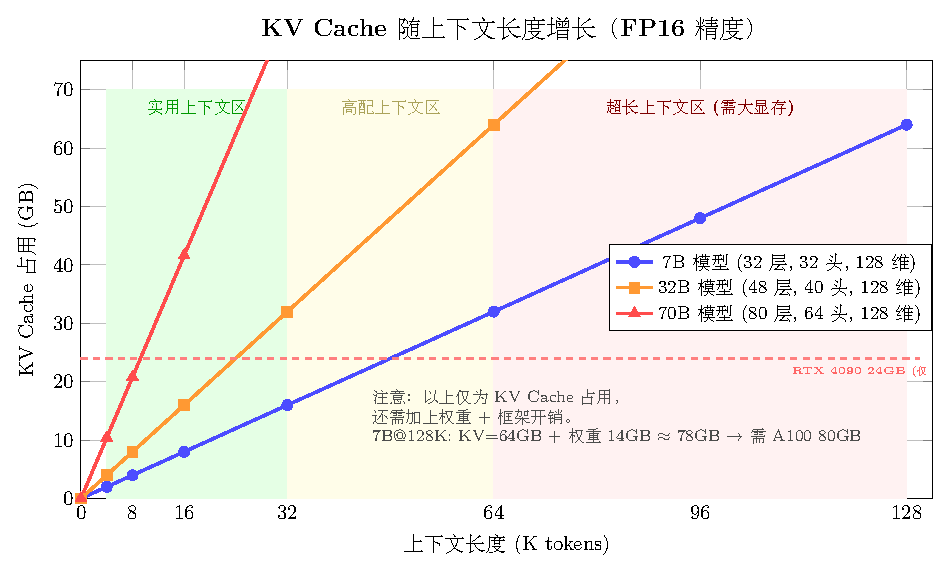
\includegraphics[width=0.75\textwidth,height=0.5\textheight,keepaspectratio]{figures/03-kvcache-vs-context.pdf}
  \end{center}
  \begin{alertblock}{关键认知}
    长上下文 = 用显存换来的，且是\textbf{超线性代价}。7B@128K 的 KV Cache 已达 64GB，足以吞没一张 RTX 4090 的全部显存。
  \end{alertblock}
\end{frame}

% -------------------- GPU 显存分解 --------------------
\begin{frame}{GPU 显存到底存什么？}
  \begin{block}{显存完整「账单」公式}
    \[
    \boxed{
    \begin{aligned}
    \text{VRAM}_{\text{total}} \approx &\ \text{参数量} \times \text{每参数字节数} \\
                                      &+ 2 \times L \times H \times D \times 2B \times \text{tokens} \\
                                      &+ \mathbf{2\text{ GB (框架开销)}}
    \end{aligned}
    }
    \]
  \end{block}

  \vspace{0.3em}
  \textbf{举例：7B FP16，8K 上下文，32层，32头，128维}
  \begin{itemize}
    \item 权重：$7\times 10^9 \times 2 = 14\text{ GB}$
    \item KV Cache：$\approx 4.3\text{ GB}$
    \item 框架开销：$\approx 2\text{ GB}$
    \item \textbf{总计：约 20--22 GB}
  \end{itemize}

  \vspace{0.3em}
  \begin{keypoint}
    7B FP16 @ 8K 上下文，\textbf{至少需要 24 GB 显存}（RTX 4090 / 3090）。
  \end{keypoint}
\end{frame}

\begin{frame}{显存占用直观分解}
  \begin{center}
    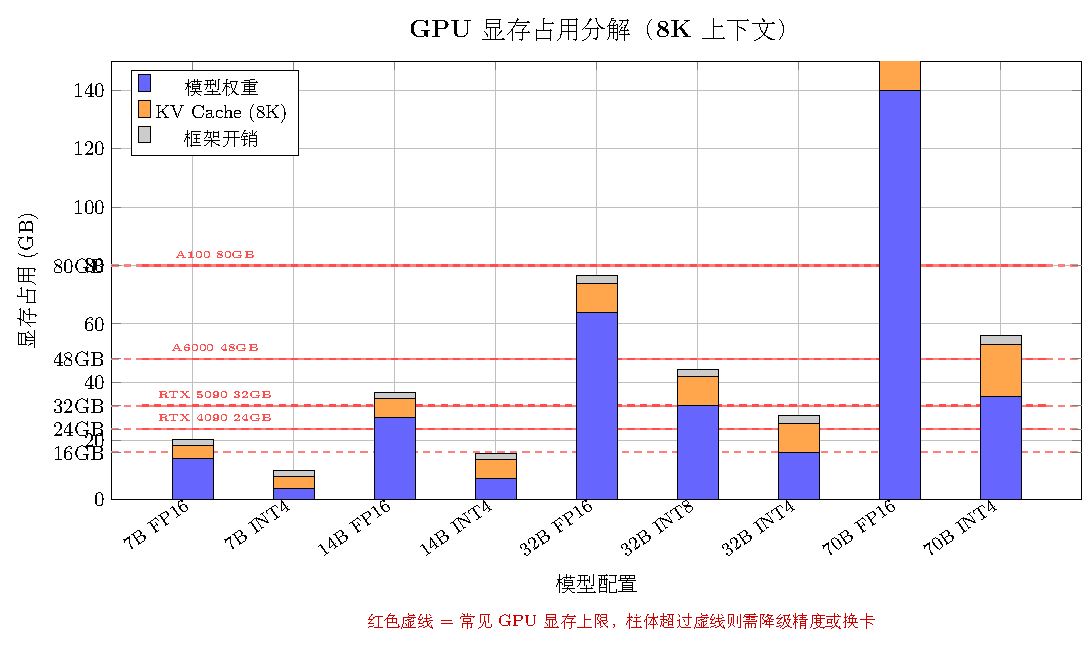
\includegraphics[width=0.75\textwidth,height=0.5\textheight,keepaspectratio]{figures/01-gpu-vram-breakdown.pdf}
  \end{center}
  \begin{alertblock}{红色虚线 = 常见 GPU 显存上限}
    柱体超过虚线 = 必须降低精度或换 GPU
  \end{alertblock}
\end{frame}

% -------------------- 量化 --------------------
\begin{frame}{量化 (Quantization) 的本质}
  \begin{columns}[T]
    \column{0.45\textwidth}
    \textbf{精度格式与显存占用}
    \begin{itemize}
      \item \textbf{FP16/BF16}：2 bytes/参数，标准推理精度
      \item \textbf{INT8}：1 byte/参数，精度损失 $<$ 1\%
      \item \textbf{INT4}：0.5 bytes/参数，精度损失 1--3\%
      \item \textbf{GGUF (llama.cpp)}：Q2\_K 到 Q8\_0 多级量化，支持 CPU+GPU 混合
    \end{itemize}

    \column{0.52\textwidth}
    \textbf{32B 模型各精度显存需求}
    \begin{itemize}
      \item FP16：$32\times 2 = 64\text{ GB}$ — A100 80GB 或双卡
      \item INT8：$32\times 1 = 32\text{ GB}$ — 单张 A100 或 2$\times$4090
      \item INT4：$32\times 0.5 = 16\text{ GB}$ — 单张 RTX 4090
    \end{itemize}
  \end{columns}

  \vspace{0.5em}
  \begin{warningblock}
    量化只压缩权重！KV Cache 仍为 FP16。长上下文下，量化模型依然面临 KV Cache 爆炸。
  \end{warningblock}
\end{frame}

% -------------------- Prompt 为什么慢 --------------------
\begin{frame}{为什么 Prompt 越长越慢？}
  \begin{enumerate}
    \item \textbf{Prefill 阶段（计算密集）}
    \begin{itemize}
      \item 一次性计算所有输入 token 的 Attention
      \item 32K token Prompt，即使 H100 也需数秒
    \end{itemize}

    \item \textbf{Decode 阶段（显存带宽瓶颈）}
    \begin{itemize}
      \item 每生成一个新 token，需与所有历史 token 做 Attention
      \item 每次从 HBM 读取全部权重（如 7B FP16 = 14 GB）
    \end{itemize}

    \item \textbf{Attention 二次方复杂度}
    \begin{itemize}
      \item 标准因果 Attention：$O(L^2)$ 计算量
      \item Flash Attention 优化到 $O(L)$ 显存访问，但计算仍是 $O(L^2)$
    \end{itemize}
  \end{enumerate}
\end{frame}

% -------------------- 推理瓶颈 --------------------
\begin{frame}{推理瓶颈：算力 vs 显存带宽}
  \begin{center}
    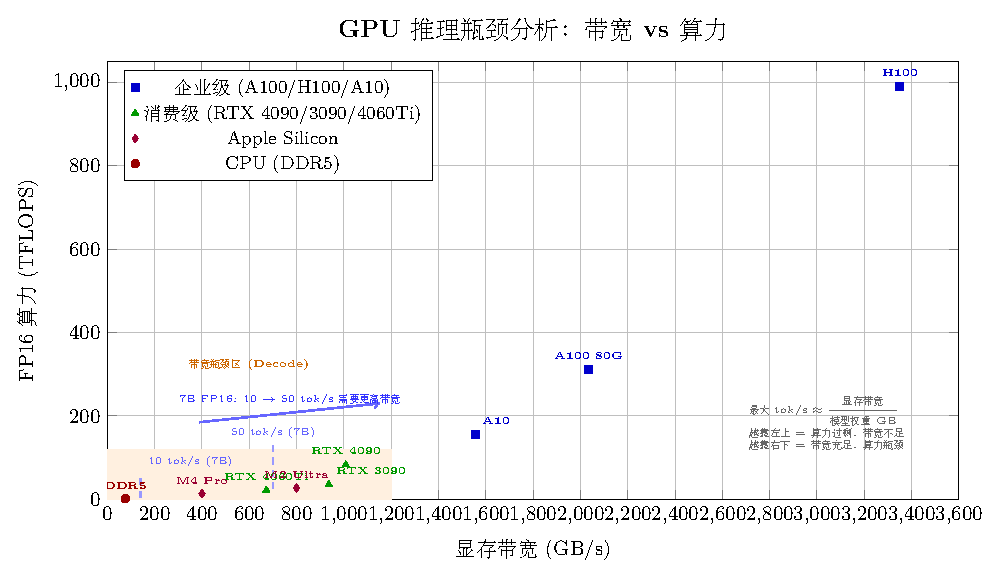
\includegraphics[width=0.7\textwidth,height=0.5\textheight,keepaspectratio]{figures/02-inference-bottleneck.pdf}
  \end{center}

  \begin{block}{核心洞察}
    \textbf{Decode 阶段瓶颈几乎总是显存带宽，而非算力。}
    \begin{itemize}
      \item 每次生成 1 token：读 14 GB 权重 $\rightarrow$ 做微小矩阵乘法 $\rightarrow$ 写 KV Cache
      \item H100 (3.35 TB/s) > A100 (2 TB/s) > RTX 4090 (1 TB/s)
      \item Apple M2 Ultra (800 GB/s 统一内存) — 推理大模型表现好的根本原因
    \end{itemize}
  \end{block}
\end{frame}

% -------------------- 企业 vs 消费 --------------------
\begin{frame}{企业级 GPU vs 消费级 GPU}
  \begin{table}
    \centering
    \begin{tabular}{p{2cm}p{4.5cm}p{3.5cm}}
      \toprule
      \textbf{维度}       & \textbf{企业级 (A100/H100)}  & \textbf{消费级 (RTX 4090)} \\
      \midrule
      显存                & 40/80 GB HBM2e/HBM3         & 24 GB GDDR6X               \\
      显存带宽            & 2--3.35 TB/s                 & 1 TB/s                     \\
      NVLink              & 有（多卡互联）              & 无                         \\
      ECC                 & 有                          & 无                         \\
      虚拟化              & MIG 支持                    & 无                         \\
      价格                & \$15K--\$35K                 & \$1.6K                     \\
      \bottomrule
    \end{tabular}
  \end{table}

  \begin{keypoint}
    企业级壁垒不在算力，在：显存 + 带宽 + 多卡互联 + ECC + 虚拟化。如不需多卡互联和高并发，RTX 4090 性价比更高。
  \end{keypoint}
\end{frame}

% -------------------- 能跑 vs 好用 --------------------
\begin{frame}{能跑 vs 好用：工程鸿沟（本文最重要概念）}
  \begin{table}
    \centering
    \begin{tabular}{p{1.8cm}p{4cm}p{5cm}}
      \toprule
      \textbf{维度}   & \textbf{能跑（Demo）}                  & \textbf{好用（Production）} \\
      \midrule
      响应速度         & 5--10 s/token（不可用）               & $>$20 tokens/s（流畅）    \\
      并发             & 1 人独占                              & 5--20 人同时使用           \\
      上下文           & 2K--4K                                & 32K--128K                  \\
      可靠性           & 偶尔 OOM 崩溃                         & 7$\times$24 稳定           \\
      量化             & Q4（有明显退化）                      & Q8 或 FP16                 \\
      RAG              & 无或简陋                              & 完整检索链路               \\
      监控             & 无                                    & GPU 利用率、延迟 P50/P99   \\
      \bottomrule
    \end{tabular}
  \end{table}

  \begin{center}
    \textbf{「7B 模型在树莓派上跑」属于能跑，不能用于生产。}
  \end{center}
\end{frame}

% ============================================================
%  第二章：主流本地部署方案调研
% ============================================================
\section{主流本地部署方案调研}

% -------------------- 模型选型总览 --------------------
\begin{frame}{开源模型生态总览}
  \begin{columns}[T]
    \column{0.48\textwidth}
    \begin{block}{通用模型}
      \begin{itemize}
        \item \textbf{Llama 3.1/3.2 (Meta)}：社区事实基准，生态最成熟，中文偏弱
        \item \textbf{Qwen 2.5 (阿里)}：中文最强，代码能力 (Coder) 优异
        \item \textbf{DeepSeek-V2/V3}：MoE 架构，顶级性能，部署门槛高
        \item \textbf{Gemma 2 (Google)}：参数效率高，商业条款需注意
      \end{itemize}
    \end{block}

    \column{0.48\textwidth}
    \begin{block}{代码专用模型}
      \begin{itemize}
        \item \textbf{Qwen2.5-Coder}：0.5B--32B，HumanEval 领先
        \item \textbf{DeepSeek-Coder-V2}：MoE，代码理解/生成极强
        \item \textbf{StarCoder2}：3B--15B，含 Verilog/SystemVerilog 训练数据
        \item \textbf{CodeLlama (Meta)}：7B--70B，生态成熟
        \item \textbf{Mistral/Mixtral}：欧洲活跃，MoE 效率高
      \end{itemize}
    \end{block}
  \end{columns}
\end{frame}

\begin{frame}{IC 设计场景模型推荐矩阵}
  \begin{table}
    \centering
    \small
    \begin{tabular}{p{2.6cm}p{3.8cm}p{2.5cm}p{2.2cm}p{2.5cm}}
      \toprule
      \textbf{场景}       & \textbf{推荐模型}             & \textbf{理由}           & \textbf{备选}                & \textbf{最小显存} \\
      \midrule
      代码补全             & Qwen2.5-Coder-7B             & 代码好，轻量            & DeepSeek-Coder-6.7B         & 16 GB            \\
      代码理解/审查        & Qwen2.5-Coder-32B            & 32B 是甜点              & DeepSeek-Coder-V2           & 24 GB (Q4)       \\
      中文文档/RAG         & Qwen2.5-14B                  & 中文最好                & Qwen2.5-32B                 & 16 GB (Q4)       \\
      通用助手             & Llama-3.1-8B                 & 生态最好                & Mistral-7B                  & 16 GB            \\
      最高代码质量         & Qwen2.5-Coder-32B / DSC-V2   & 顶级                    & —                           & 40 GB+ (FP16)     \\
      \bottomrule
    \end{tabular}
  \end{table}

  \vspace{0.5em}
  \textbf{对 IC 设计场景}：中文文档多用 Qwen，英文代码多用 DeepSeek-Coder，通用任务用 Llama。
\end{frame}

% -------------------- 推理框架 --------------------
\begin{frame}{推理框架对比（一）：入门与引擎}
  \begin{columns}[T]
    \column{0.48\textwidth}
    \begin{block}{Ollama}
      \begin{itemize}
        \item 封装 llama.cpp，Docker 式体验
        \item \texttt{ollama pull / run}
        \item 单请求队列，无生产级监控
        \item \textbf{适合}：个人实验、3--5 人小团队
      \end{itemize}
    \end{block}

    \begin{block}{llama.cpp}
      \begin{itemize}
        \item C/C++ 推理引擎，GGUF 格式
        \item CPU-GPU 混合推理
        \item Metal 加速（Apple Silicon）
        \item \textbf{适合}：本地部署基础层
      \end{itemize}
    \end{block}

    \column{0.48\textwidth}
    \begin{block}{vLLM（生产首选）}
      \begin{itemize}
        \item \textbf{PagedAttention}：KV Cache 利用率 $\approx$ 100\%
        \item \textbf{Continuous Batching}
        \item OpenAI API 兼容
        \item 张量并行、前缀缓存
        \item \textbf{适合}：企业多用户部署
      \end{itemize}
    \end{block}

    \begin{block}{SGLang（新一代）}
      \begin{itemize}
        \item RadixAttention（前缀缓存更高效）
        \item 结构化生成（JSON 模式约束）
        \item 部分基准比 vLLM 快 2--5$\times$
        \item \textbf{适合}：延迟敏感 + 结构化输出
      \end{itemize}
    \end{block}
  \end{columns}
\end{frame}

\begin{frame}{推理框架对比（二）：极致性能与前端}
  \begin{columns}[T]
    \column{0.48\textwidth}
    \begin{block}{TensorRT-LLM (NVIDIA)}
      \begin{itemize}
        \item 性能天花板最高（vs vLLM 2--4$\times$）
        \item FP8 (H100)、In-flight Batching
        \item 部署复杂，依赖 NVIDIA 生态
        \item \textbf{适合}：极致性能 + 企业级 GPU
      \end{itemize}
    \end{block}

    \begin{block}{HuggingFace TGI}
      \begin{itemize}
        \item 功能与 vLLM 类似
        \item 深度绑定 HuggingFace Hub
        \item HF 自用生产，成熟度有保障
      \end{itemize}
    \end{block}

    \column{0.48\textwidth}
    \begin{block}{前端工具（非推理引擎）}
      \begin{itemize}
        \item \textbf{Open WebUI}：类 ChatGPT Web 界面
        \item \textbf{Continue.dev}：IDE 插件，行内补全
        \item \textbf{LM Studio}：图形化下载/管理模型
        \item \textbf{AnythingLLM}：内置 RAG 客户端
      \end{itemize}
    \end{block}
  \end{columns}
\end{frame}

\begin{frame}{框架推荐矩阵}
  \begin{table}
    \centering
    \begin{tabular}{p{2.2cm}p{4cm}p{3cm}p{3cm}}
      \toprule
      \textbf{场景}           & \textbf{推荐框架}           & \textbf{理由}          & \textbf{备选} \\
      \midrule
      个人实验               & Ollama + Open WebUI        & 5 分钟上手             & LM Studio    \\
      3--10 人团队            & vLLM + Open WebUI          & 并发支持好             & Ollama       \\
      生产部署               & vLLM 或 SGLang             & 工业级稳定             & TensorRT-LLM \\
      Apple Silicon          & llama.cpp + Ollama         & Metal 加速最好         & —            \\
      NVIDIA 多卡            & vLLM（张量并行）           & 开箱即用               & TensorRT-LLM \\
      \bottomrule
    \end{tabular}
  \end{table}
\end{frame}

\begin{frame}{推理框架生态全景}
  \begin{center}
    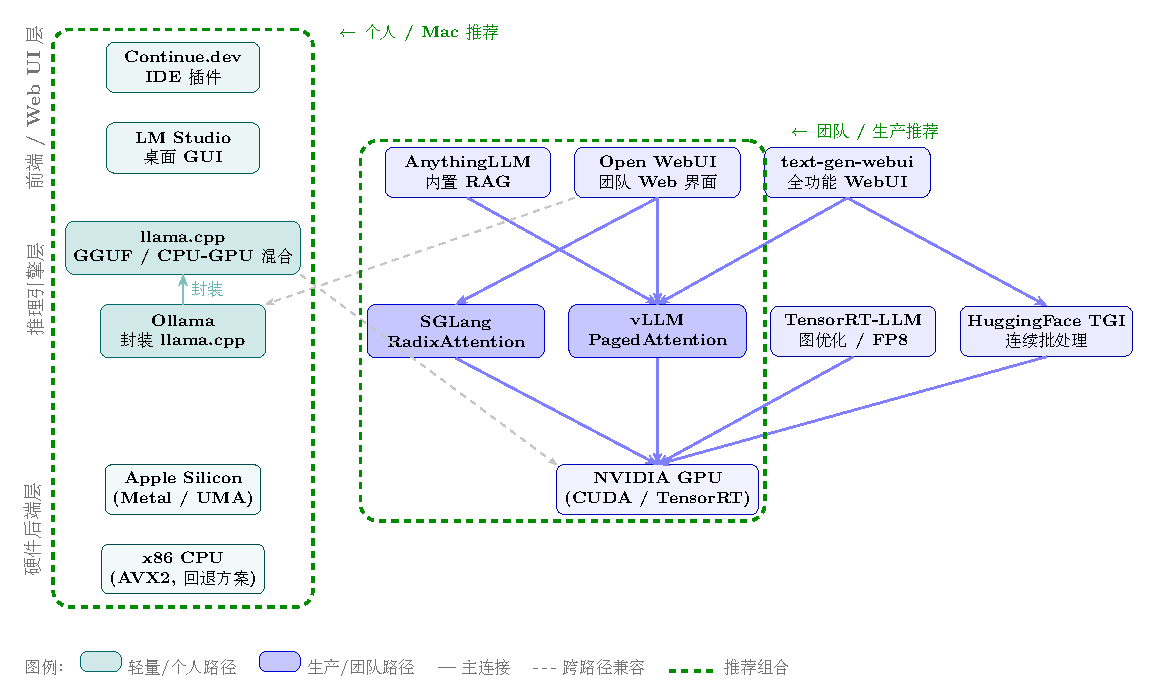
\includegraphics[width=0.8\textwidth,height=0.55\textheight,keepaspectratio]{figures/04-framework-ecosystem.pdf}
  \end{center}
  \begin{center}
    \textbf{推荐组合（绿色虚线）：Continue.dev + vLLM 或 Open WebUI + Ollama}
  \end{center}
\end{frame}

% ============================================================
%  第三章：最低资源验证可行性
% ============================================================
\section{如果只是验证可行性，最少需要什么？}

\begin{frame}{PoC（概念验证，Proof of Concept） 硬件分水岭}
  \small
  \begin{table}
    \centering
    \begin{tabular}{p{2.8cm}p{6cm}p{1.5cm}p{2.0cm}}
      \toprule
      \textbf{级别}                & \textbf{能启动}                           & \textbf{能用}                        & \textbf{推荐} \\
      \midrule
      CPU-only                    & 32GB RAM, 7B Q4, 2--5 tok/s             & 不可用                               & 不推荐        \\
      Mac Mini M4 Pro             & 24GB, 7B Q4, 15--25 tok/s               & 勉强可用                             & 个人实验      \\
      RTX 4060 Ti 16GB            & 7B Q4, 8K ctx                           & 单人勉强                             & 低预算起步    \\
      \rowcolor{green!15}
      \textbf{RTX 4090 24GB}      & 14B Q4 / 32B Q4, 32K ctx, 30--50 tok/s  & \textbf{可用}                        & \textbf{甜点} \\
      RTX 5090 32GB               & 32B Q4 / 14B FP16, 64K ctx              & \textbf{好用}                        & 高性能甜点    \\
      2$\times$RTX 4090           & 70B Q4, 张量并行, 32K ctx               & 团队可用                             & 团队起步      \\
      A100 80GB                   & 70B FP16, 128K ctx, 高并发              & 生产就绪                             & 正式部署      \\
      \bottomrule
    \end{tabular}
  \end{table}
\end{frame}

\begin{frame}{PoC 三个层次}
  \begin{columns}[T]
    \column{0.32\textwidth}
    \begin{block}{层次一：零成本（0 元, 0 天）}
      \begin{itemize}
        \item 现有 MacBook Pro 或开发服务器
        \item Ollama + Qwen2.5-Coder-7B-Q4
        \item Continue.dev IDE 补全
        \item \textbf{只能确认方向，不能用于决策}
      \end{itemize}
    \end{block}

    \column{0.32\textwidth}
    \begin{alertblock}{层次二：低成本 PoC（\textasciitilde ¥15K, 1--2 天）}
      \textbf{甜点方案！}
      \begin{itemize}
        \item RTX 4090 24GB + 64GB RAM
        \item vLLM + Qwen2.5-Coder-32B-Q4
        \item 32K 上下文
        \item 3--5 人试用 2--4 周
        \item \textbf{足以决策}
      \end{itemize}
    \end{alertblock}

    \column{0.32\textwidth}
    \begin{block}{层次三：准生产 PoC（\textasciitilde ¥60K--¥120K）}
      \begin{itemize}
        \item 2$\times$RTX 4090/5090 + 128GB
        \item vLLM 张量并行
        \item Qwen2.5-72B-Q4 / DSC-V2
        \item 128K 长上下文
        \item 10--20 人团队
      \end{itemize}
    \end{block}
  \end{columns}
\end{frame}

\begin{frame}{Mac Mini 是否够？}
  \begin{alertblock}{坦白说：对于企业 PoC，不推荐 Mac Mini}
    \begin{itemize}
      \item M4 Pro Mac mini 64GB 统一内存（约 ¥20K+）——不如二手 RTX 4090 工作站
      \item Metal 加速在 vLLM/SGLang 等生产框架中支持不完善
      \item 无法扩展到多卡/多机
      \item 企业中最终还是 Linux + NVIDIA，PoC 阶段就应用最终平台
    \end{itemize}
  \end{alertblock}

  \vspace{0.3em}
  \textbf{唯一例外}：已有 Mac Studio M2 Ultra 192GB，可顺手跑 PoC——但不应「为此购买」。
\end{frame}

\begin{frame}{PoC 方案成本对比}
  \small
  \begin{table}
    \centering
    \begin{tabular}{p{4.5cm}p{1.5cm}p{1.5cm}p{1.5cm}p{1.8cm}p{1.5cm}}
      \toprule
      \textbf{方案}                 & \textbf{硬件成本} & \textbf{满载功耗} & \textbf{月电费} & \textbf{模型}   & \textbf{速度} \\
      \midrule
      MacBook Pro M4 Pro 24GB       & ¥18K     & 30W             & ¥17             & 7B Q4           & 15--20 t/s    \\
      \rowcolor{green!15}
      RTX 4090 工作站               & ¥25K             & 500W            & ¥288            & 32B Q4          & 30--50 t/s    \\
      2$\times$RTX 4090              & ¥40K             & 800W            & ¥460            & 70B Q4          & 15--25 t/s    \\
      A100 80GB 二手               & ¥50K             & 400W            & ¥230            & 70B FP16        & 40--60 t/s    \\
      \bottomrule
    \end{tabular}
  \end{table}

  \vspace{0.3em}
  \begin{keypoint}
    自建 RTX 4090 方案在 3 个月内回本（对比云 GPU 月费 ¥5K--¥8K）。
  \end{keypoint}
\end{frame}

% ============================================================
%  第四章：IC 设计场景中的真实落地方式
% ============================================================
\section{IC 设计场景中的真实落地}

\begin{frame}{IC 设计流程 LLM 介入全景}
  \begin{center}
    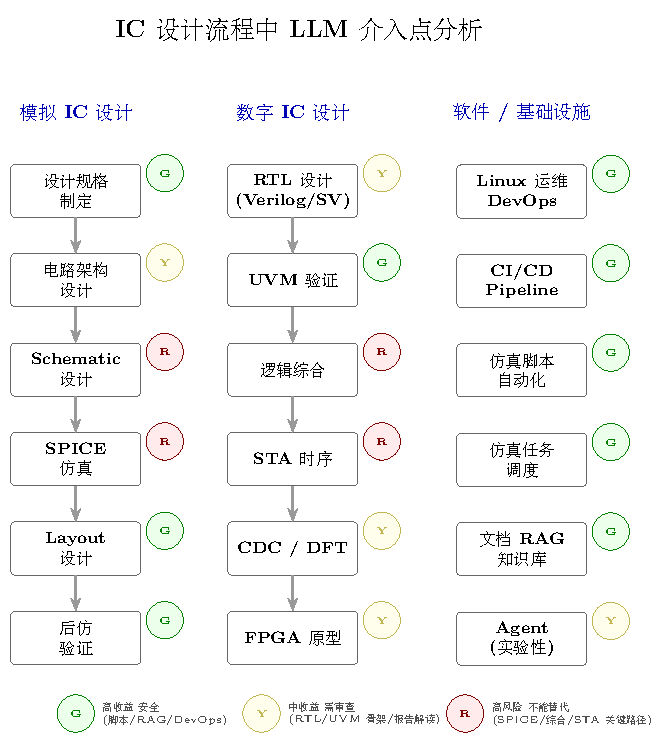
\includegraphics[width=0.8\textwidth,height=0.45\textheight,keepaspectratio]{figures/05-ic-flow-llm-intervention.pdf}
  \end{center}

  \begin{itemize}
    \item \textcolor{darkgreen}{● 绿色(G)} = 高收益安全区：脚本/RAG/DevOps
    \item \textcolor{gold}{● 黄色(Y)} = 中收益需审查：RTL 骨架/报告解读
    \item \textcolor{darkred}{● 红色(R)} = 高风险不能替代：SPICE/综合/STA 关键路径
  \end{itemize}
\end{frame}

% -------------------- 模拟 IC --------------------
\begin{frame}{模拟 IC 设计：电路与架构 ★★☆☆☆}
  \begin{columns}[T]
    \column{0.5\textwidth}
    \begin{block}{能做什么 ✓}
      \begin{itemize}
        \item 读网表，解释电路拓扑
        \item 识别常见结构：Bandgap、运放、比较器、LDO
        \item 提供经典架构参考
        \item 解释设计公式和 trade-off
        \item 生成仿真 testbench 骨架
      \end{itemize}
    \end{block}

    \column{0.5\textwidth}
    \begin{alertblock}{不能做什么 ✗（危险区域）}
      \begin{itemize}
        \item \textbf{不能替代 SPICE 仿真}——LLM 不知物理
        \item 不了解具体工艺 PDK
        \item 高频/RF EM 效应无法处理
        \item SerDes CDR/DFE/CTLE 参数——核心 IP，无训练数据
      \end{itemize}
    \end{alertblock}
  \end{columns}

  \vspace{0.3em}
  架构参考有用，设计迭代必须靠仿真和工程师经验。
\end{frame}

\begin{frame}{模拟 IC 设计：脚本与工具链 ★★★★★}
  \begin{block}{模拟 IC 中 LLM 收益最高的场景}
    \begin{itemize}
      \item 生成 Cadence Skill/Ocean 脚本 — 文档稀缺，AI 辅助编写价值巨大
      \item 生成 HSPICE/Spectre 仿真 deck
      \item 生成 Python/Matlab 数据处理脚本
      \item 生成 Perl/Tcl EDA 流程自动化脚本
      \item Corner 扫描和 Monte Carlo 自动化脚本
    \end{itemize}
  \end{block}

  \vspace{0.3em}
  \begin{keypoint}
    脚本自动化是\textbf{最安全的 AI 应用场景}：出错不会导致芯片失效，容易验证。
  \end{keypoint}
\end{frame}

% -------------------- 数字 IC --------------------
\begin{frame}{数字 IC 设计：RTL 代码 ★★★☆☆}
  \begin{columns}[T]
    \column{0.5\textwidth}
    \begin{block}{能做什么 ✓}
      \begin{itemize}
        \item 根据规格生成 RTL 模块骨架
        \item 生成 FSM 的 RTL 实现
        \item 阅读现有 RTL，解释功能
        \item 识别代码风格问题
        \item 生成同步 FIFO、CDC 结构、握手协议
      \end{itemize}
    \end{block}

    \column{0.5\textwidth}
    \begin{alertblock}{不能做什么 ✗}
      \begin{itemize}
        \item 生成 RTL 不能直接综合（须审查时序/面积/功耗）
        \item 不理解综合约束（clock gating, retiming, pipeline balance）
        \item CDC 容易出错——数字设计最危险区域
        \item 不理解 SDC（false path, multicycle path）
      \end{itemize}
    \end{alertblock}
  \end{columns}

  \vspace{0.3em}
  RTL 骨架有用，\textbf{必须人工审查}。
\end{frame}

\begin{frame}{数字 IC 设计：UVM 验证 ★★★★☆}
  \begin{block}{UVM 是数字 IC 中 LLM 收益最高的场景}
    \begin{itemize}
      \item 根据接口定义自动生成 UVM driver/monitor/scoreboard 骨架
      \item 生成 UVM sequence、virtual sequence
      \item 根据 spec 生成 SystemVerilog Assertion (SVA)
      \item 生成 UVM register model（从 IP-XACT 或寄存器表）
      \item 生成 coverage model（covergroup, coverpoint, cross coverage）
    \end{itemize}
  \end{block}

  \vspace{0.3em}
  \begin{keypoint}
    UVM 模板代码量大、重复性高——\textbf{这正是 LLM 擅长的事}。\\
    SVA 语法复杂、容易写错——LLM 辅助可降低门槛。\\
    风险：可能生成「看起来对但测不到关键场景」的 testbench。
  \end{keypoint}
\end{frame}

\begin{frame}{软件/基础设施场景}
  \begin{columns}[T]
    \column{0.5\textwidth}
    \begin{block}{Linux 运维与 DevOps ★★★★★}
      \begin{itemize}
        \item Shell/Python 自动化脚本
        \item Dockerfile, docker-compose.yml
        \item CI/CD 流水线（Jenkins, GitLab CI, GitHub Actions）
        \item Ansible/Terraform 配置
        \item Log 排错与修复建议
      \end{itemize}
    \end{block}

    \column{0.5\textwidth}
    \begin{block}{仿真任务调度 ★★★★☆}
      \begin{itemize}
        \item LSF/SGE/Slurm 任务提交脚本
        \item Regression 管理脚本
        \item 仿真结果自动汇总
        \item PASS/FAIL 汇总、覆盖率趋势报告
      \end{itemize}
    \end{block}
  \end{columns}

  \vspace{0.5em}
  \begin{keypoint}
    运维自动化是 LLM 最强的通用能力。跨团队最高收益场景。
  \end{keypoint}
\end{frame}

% -------------------- RAG --------------------
\begin{frame}{为什么 RAG 对企业特别重要？}
  \begin{columns}[T]
    \column{0.48\textwidth}
    \begin{alertblock}{模型不知道的内部知识}
      \begin{itemize}
        \item 内部 IP 使用手册
        \item 内部 Bug 数据库
        \item Tapeout checklist
        \item 内部仿真环境和脚本
        \item Foundry PDK 文档（部分机密）
      \end{itemize}
    \end{alertblock}

    \column{0.48\textwidth}
    \begin{block}{为什么不能仅靠模型参数记忆？}
      \begin{itemize}
        \item 压缩是有损的——细节会丢失
        \item 无法区分记忆中的正确/错误信息
        \item 「知识截止日期」——训练后发布的文档不知道
        \item \textbf{幻觉 (Hallucination)}：编造看似合理的答案
      \end{itemize}
    \end{block}
  \end{columns}

  \vspace{0.3em}
  \begin{center}
    \textbf{RAG 核心价值：让模型基于「检索到的真实文档」回答，而非基于「参数记忆」。}
  \end{center}
\end{frame}

\begin{frame}{向量数据库的工作原理}
  \begin{center}
    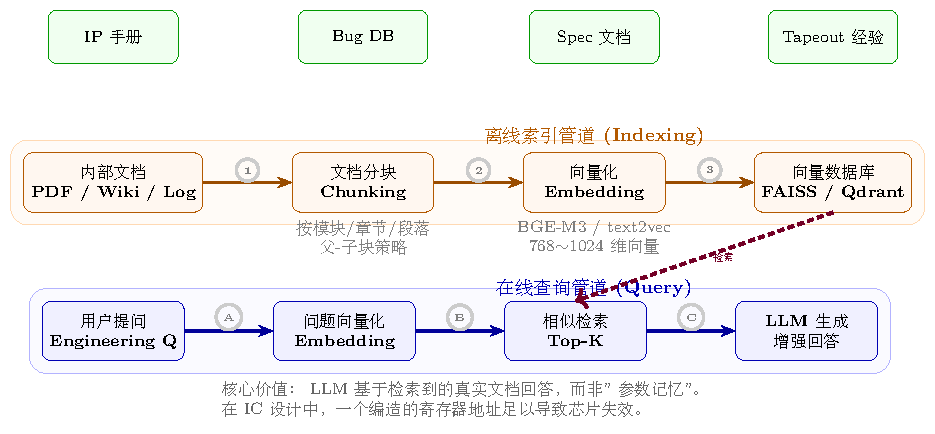
\includegraphics[width=0.75\textwidth,height=0.5\textheight,keepaspectratio]{figures/06-rag-pipeline.pdf}
  \end{center}
  \begin{enumerate}
    \item \textbf{文档分块}：长文档 $\rightarrow$ 小块（256--1024 tokens）
    \item \textbf{向量化}：Embedding 模型 $\rightarrow$ 固定维度向量（768/1024 维）
    \item \textbf{存储索引}：向量数据库 + HNSW/IVF 索引
    \item \textbf{检索}：问题向量化 $\rightarrow$ 找最相似 K 个块（K=3--10）
    \item \textbf{增强生成}：文档块作为上下文 + 问题 $\rightarrow$ LLM 生成答案
  \end{enumerate}
\end{frame}

\begin{frame}{Embedding 与 Chunking 策略}
  \begin{columns}[T]
    \column{0.48\textwidth}
    \begin{block}{Embedding：语义映射}
      \begin{itemize}
        \item 「时钟域交叉」↔「CDC」→ 相近向量
        \item 「Bandgap 温度系数」↔「TC」→ 相近向量
        \item 推荐：BGE-M3 或 text2vec-large-chinese（多语言）
      \end{itemize}
    \end{block}

    \column{0.48\textwidth}
    \begin{block}{Chunking：最被低估的环节}
      \begin{itemize}
        \item Verilog 代码块不能切断（语法完整性）
        \item 寄存器表需特殊处理
        \item 公式不能中途截断
        \item \textbf{策略}：代码按模块边界，Spec 按章节，笔记按段落
        \item 父子块：检索小粒度，返回大粒度上下文
      \end{itemize}
    \end{block}
  \end{columns}
\end{frame}

\begin{frame}{向量数据库方案对比}
  \small
  \begin{table}
    \centering
    \begin{tabular}{p{2.2cm}p{4cm}p{3.2cm}p{1cm}p{1cm}}
      \toprule
      \textbf{方案}    & \textbf{适合场景}            & \textbf{部署复杂度}    & \textbf{性能} & \textbf{社区} \\
      \midrule
      FAISS (Meta)    & 研究/PoC，单机              & 极低（Python 库）    & 极高          & 活跃         \\
      Chroma          & 小团队 PoC                  & 极低                 & 中等          & 活跃         \\
      Qdrant          & 企业生产                    & 中（Rust, 单二进制）  & 高            & 活跃         \\
      pgvector        & 已有 PostgreSQL 的团队      & 低（PG 插件）        & 中等          & 活跃         \\
      Elasticsearch   & 已有 ES 的团队              & 低（已有基础设施）    & 中等          & 成熟         \\
      Milvus          & 企业生产                    & 中高（etcd/MinIO等） & 高            & 活跃         \\
      \bottomrule
    \end{tabular}
  \end{table}

  \begin{block}{推荐}
    PoC 阶段：Chroma 或 FAISS；生产阶段：Qdrant 或 pgvector。\\
    \textbf{不推荐 Milvus 给初创}——依赖太多（etcd + MinIO + Pulsar），运维负担过重。
  \end{block}
\end{frame}

% ============================================================
%  第五章：Agent 在 IC 设计中的可能性
% ============================================================
\section{Agent 在 IC 设计中的可能性}

\begin{frame}{什么是 AI Agent？}
  \begin{center}
    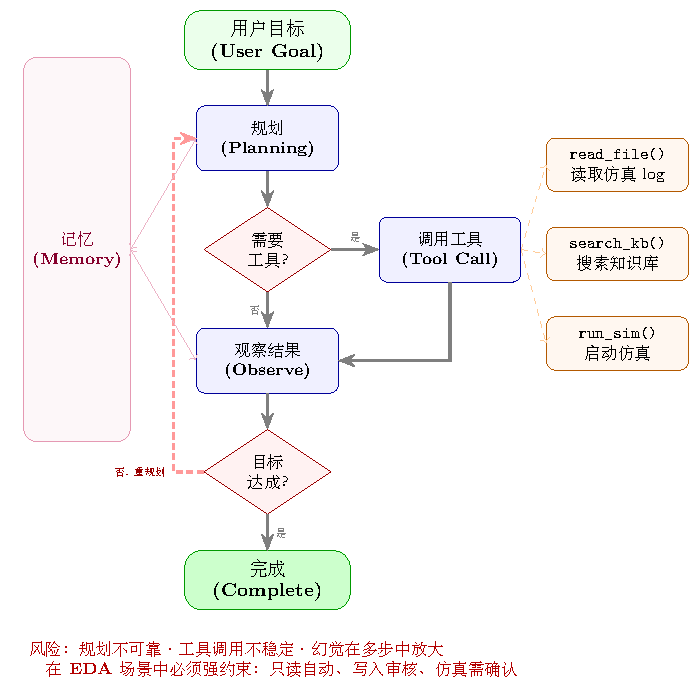
\includegraphics[width=0.65\textwidth,height=0.45\textheight,keepaspectratio]{figures/07-agent-loop.pdf}
  \end{center}

  \[
  \boxed{\text{AI Agent} = \text{LLM} + \text{Tool Calling} + \text{Planning} + \text{Memory} + \text{执行循环}}
  \]

  \begin{enumerate}
    \item 用户目标 → Agent 规划步骤 → 调用工具 → 观察结果 → 调整计划 → 循环至完成
  \end{enumerate}
\end{frame}

\begin{frame}{Agent 的核心能力与风险}
  \begin{columns}[T]
    \column{0.48\textwidth}
    \begin{block}{核心能力}
      \begin{itemize}
        \item \textbf{Tool Calling}：LLM 决定调用哪个工具并生成参数
        \item \textbf{MCP (Model Context Protocol)}：标准化协议，类比 USB-C 之于外设
        \item \textbf{Workflow Engine}：LangGraph, Prefect, Temporal
        \item 支持条件分支、并行执行、错误重试、人工审核节点
      \end{itemize}
    \end{block}

    \column{0.48\textwidth}
    \begin{alertblock}{为什么 Agent 容易失控}
      \begin{enumerate}
        \item 规划不可靠（概率性预测 $\neq$ 逻辑推理）
        \item 工具调用不稳定（错误参数、遗漏步骤）
        \item 幻觉在多步骤中累积放大
        \item 缺乏领域知识（不知什么是「危险操作」）
        \item 无成本意识（可能反复启动昂贵仿真）
      \end{enumerate}
    \end{alertblock}
  \end{columns}
\end{frame}

\begin{frame}{EDA 场景的 Agent 安全边界}
  \begin{center}
    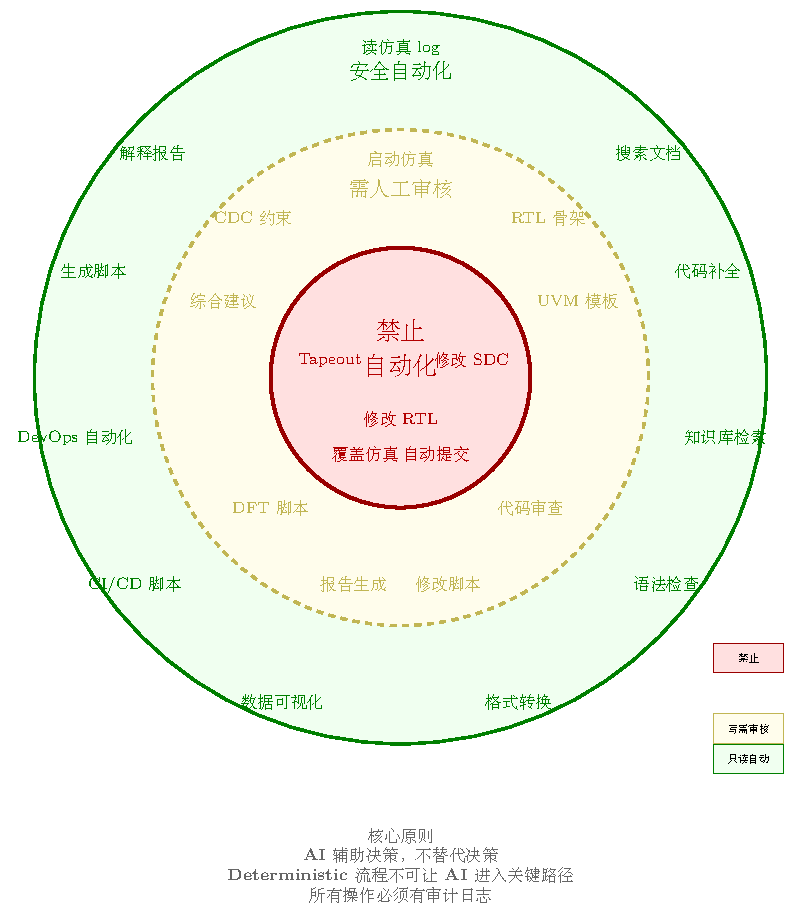
\includegraphics[width=0.7\textwidth,height=0.45\textheight,keepaspectratio]{figures/08-agent-safety-boundary.pdf}
  \end{center}

  \begin{itemize}
    \item \textcolor{darkgreen}{● 绿圈} = 只读自动化（安全）：读 log、读报告、搜索文档
    \item \textcolor{gold}{● 黄圈} = 写入需人工审核：修改 constraint/RTL/提交代码
    \item \textcolor{darkred}{● 红圈} = 禁止自动化：自动修改 tapeout 数据
  \end{itemize}

  \vspace{0.3em}
  \begin{keypoint}
    核心原则：\textbf{AI 辅助决策，而非替代决策。}不要放在确定性流程的关键路径上。
  \end{keypoint}
\end{frame}

\begin{frame}{当前可行的 Agent 场景}
  \begin{columns}[T]
    \column{0.5\textwidth}
    \begin{block}{可行（低风险，高收益）}
      \begin{itemize}
        \item \textbf{仿真 Log 分析 Agent}：自动读 regression log，分类错误，给出初步分析
        \item \textbf{文档问答 Agent}：RAG + Agent 搜索内部文档回答技术问题
        \item \textbf{仿真报告生成 Agent}：自动收集结果、画图、生成 summary
      \end{itemize}
    \end{block}

    \column{0.5\textwidth}
    \begin{alertblock}{当前不适合（高风险）}
      \begin{itemize}
        \item \textbf{自动修改 RTL}：风险太高
        \item \textbf{自动修改 constraint}：风险太高
        \item \textbf{自动决定 tapeout 参数}：绝对不行
      \end{itemize}
    \end{alertblock}
  \end{columns}

  \vspace{0.5em}
  代码审查 Agent（中风险，中收益）：读取 PR diff，对照 coding guideline 提建议。
\end{frame}

% ============================================================
%  第六章：最终建议方案
% ============================================================
\section{最终建议方案}

% -------------------- 方案 A --------------------
\begin{frame}{方案 A：最低成本 PoC（¥25K--¥35K）}
  \small
  \begin{columns}[T]
    \column{0.45\textwidth}
    \begin{block}{硬件配置}
      \begin{itemize}
        \item \textbf{GPU}：1$\times$RTX 4090 24GB（约 ¥13K）
        \item \textbf{CPU}：Ryzen 9 7950X 或 i9-14900K
        \item \textbf{RAM}：64GB DDR5
        \item \textbf{存储}：2TB NVMe SSD
        \item \textbf{电源}：1000W 80+ Gold
        \item \textbf{OS}：Ubuntu 24.04 LTS
      \end{itemize}
    \end{block}

    \column{0.52\textwidth}
    \begin{block}{软件栈}
      \begin{itemize}
        \item \textbf{推理框架}：vLLM（生产级）+ Ollama（备用）
        \item \textbf{模型}：Qwen2.5-Coder-14B-Q4 / 32B-Q4
        \item \textbf{RAG}：Chroma + BGE-M3 Embedding
        \item \textbf{Web UI}：Open WebUI
        \item \textbf{监控}：nvitop + Prometheus + Grafana
      \end{itemize}
    \end{block}
  \end{columns}

  \vspace{0.3em}
  \textbf{能力}：3--8 人同时使用，32K 上下文，20--50 tok/s（单用户）。\\
  \textbf{风险}：单卡无冗余，24GB 显存限制模型选择上限，无 ECC。
\end{frame}

% -------------------- 方案 B --------------------
\begin{frame}{方案 B：初创公司推荐方案（¥60K--¥100K）}
  \small
  \begin{columns}[T]
    \column{0.45\textwidth}
    \begin{block}{硬件配置}
      \begin{itemize}
        \item \textbf{GPU}：2$\times$RTX 4090 或 1$\times$RTX 5090 32GB
        \item \textbf{CPU}：Threadripper 或 Xeon W
        \item \textbf{RAM}：128GB DDR5
        \item \textbf{存储}：4TB NVMe + 8TB 备份（HDD/SSD）
        \item \textbf{OS}：Ubuntu 24.04 LTS
      \end{itemize}
    \end{block}

    \column{0.52\textwidth}
    \begin{block}{软件栈}
      \begin{itemize}
        \item \textbf{推理框架}：vLLM（张量并行）+ SGLang（结构化输出）
        \item \textbf{主力模型}：Qwen2.5-Coder-32B-Q4
        \item \textbf{高级模型}：Qwen2.5-72B-Q4
        \item \textbf{RAG}：Qdrant + BGE-M3 / text2vec-large-chinese
        \item \textbf{Agent}：LangChain/LangGraph（实验性）
        \item \textbf{监控}：Grafana + Loki + Prometheus
      \end{itemize}
    \end{block}
  \end{columns}

  \vspace{0.3em}
  \textbf{能力}：10--20 人，64K--128K 上下文，完整 RAG，Agent 原型。\\
  \textbf{注意}：不需要 K8s（过度设计），不需要 InfiniBand/NVLink（PCIe 4.0 足够 2--4 卡）。
\end{frame}

% -------------------- 方案 C --------------------
\begin{frame}{方案 C：长期企业化演进（1--3 年）}
  \begin{center}
    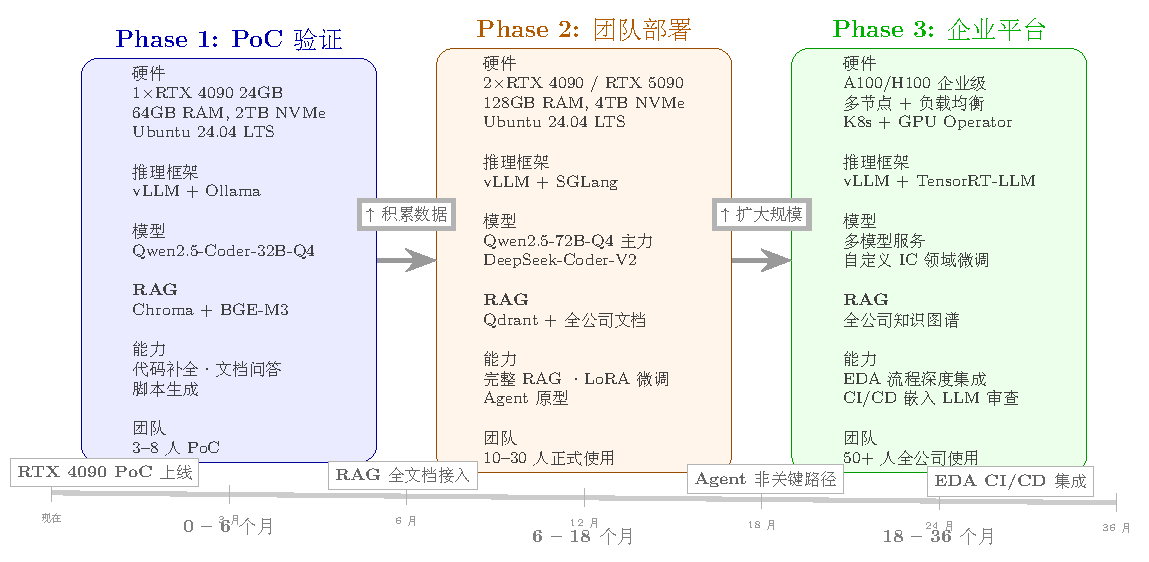
\includegraphics[width=0.8\textwidth,height=0.5\textheight,keepaspectratio]{figures/09-evolution-roadmap.pdf}
  \end{center}

  \begin{columns}[T]
    \column{0.32\textwidth}
    \textbf{Phase 1 (0--6月)}\\
    方案 B，单机双卡，积累使用数据

    \column{0.32\textwidth}
    \textbf{Phase 2 (6--18月)}\\
    企业级 GPU（A100/H100），RAG 知识库，微调（LoRA），Agent 非关键路径

    \column{0.32\textwidth}
    \textbf{Phase 3 (18--36月)}\\
    多节点 + K8s + 负载均衡，与 EDA 深度集成，自定义 IC 领域模型
  \end{columns}
\end{frame}

% -------------------- 买硬件 vs 云 --------------------
\begin{frame}{关键决策：买硬件 vs 用云}
  \begin{table}
    \centering
    \begin{tabular}{p{3cm}p{3.5cm}p{4.5cm}}
      \toprule
      \textbf{维度}     & \textbf{自建（RTX 4090）}    & \textbf{云 GPU（A10 等效）} \\
      \midrule
      硬件成本           & ¥13K（一次性）              & ¥0                         \\
      月费               & ¥300（电费）                & ¥5K--¥8K（24/7）          \\
      回本周期           & —                           & \textbf{2--3 个月}          \\
      数据安全           & 完全本地                    & 需评估（VPC 内可接受）      \\
      运维               & 需要 Linux 基础             & 云厂商负责                  \\
      扩展性             & 有限（加卡即可）            & 弹性                        \\
      \bottomrule
    \end{tabular}
  \end{table}

  \begin{keypoint}
    对初创 IC 公司：\textbf{自建方案在 3 个月内回本}。代码和数据是核心资产，本地部署更安全。
  \end{keypoint}
\end{frame}

% -------------------- 优先级排序 --------------------
\begin{frame}{哪些方向最值得投入？（优先级排序）}
  \begin{center}
    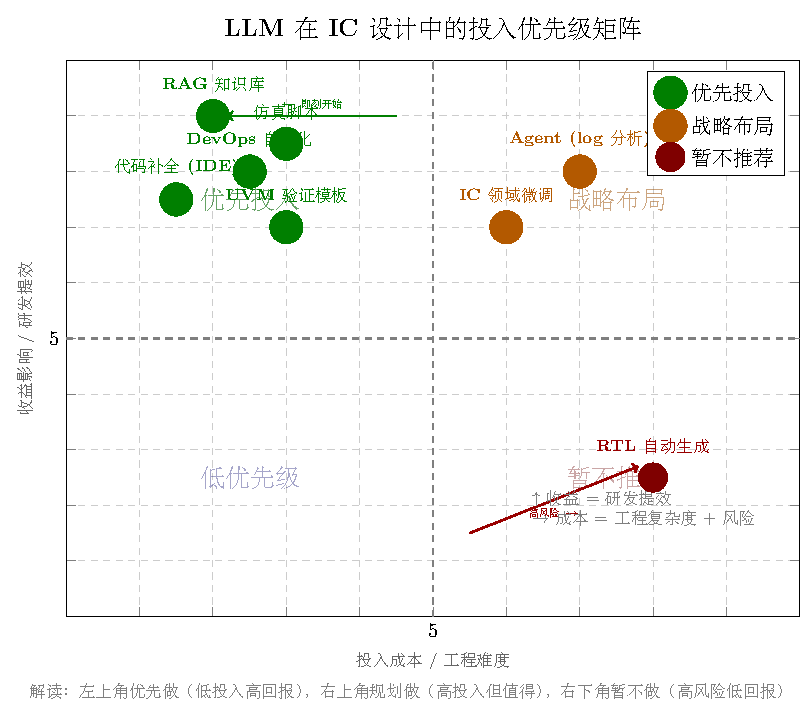
\includegraphics[width=0.65\textwidth,height=0.45\textheight,keepaspectratio]{figures/10-priority-matrix.pdf}
  \end{center}

  \begin{enumerate}
    \item \textbf{RAG 知识库建设}（最高优先级，即刻开始）— 投入产出比最高
    \item \textbf{代码补全（IDE 集成）}（高优先级）— 工程师每天可感受到的提效
    \item \textbf{UVM/验证自动化}（高优先级）— 验证代码量大且模式化
    \item \textbf{脚本/DevOps 自动化}（高优先级）— 安全、高效、通用
    \item \textbf{Agent（log 分析/报告）}（中优先级）— 非关键路径实验
    \item \textbf{微调 Fine-tuning}（中低优先级）— 积累够 IC 领域数据后再做
    \item \textbf{RTL 自动生成}（低优先级，高风险）— 当前不推荐
  \end{enumerate}
\end{frame}

% -------------------- AI 幻觉 vs 未来 --------------------
\begin{frame}{哪些方向现在只是「AI 幻觉」？}
  \begin{alertblock}{这些不是工程，是科幻}
    \begin{itemize}
      \item \textbf{「AI 自动设计芯片」}：芯片涉及物理约束、工艺特性、多物理场仿真，LLM 无法替代
      \item \textbf{「AI 替代 SPICE 仿真」}：SPICE 解微分方程，LLM 做概率性 token 预测——本质不同
      \item \textbf{「AI 自动发现新电路拓扑」}：目前没有可信证据
      \item \textbf{「AI 替代资深工程师」}：AI 是工具，放大工程师能力，不是替代判断
    \end{itemize}
  \end{alertblock}

  \vspace{0.5em}
  \begin{block}{未来 3--5 年可能成熟}
    \begin{itemize}
      \item 多模态 EDA AI（「看懂」电路图/波形图/Layout）
      \item EDA 专用代码模型（理解时序/面积/功耗约束）
      \item 可信任 EDA Agent（安全边界内设计空间探索）
      \item AI 辅助模拟电路优化（Bayesian Optimization + LLM）
    \end{itemize}
  \end{block}
\end{frame}

% -------------------- 核心结论 --------------------
\begin{frame}{最关键的竞争壁垒是什么？}
  \begin{tikzpicture}
    \node[draw=red!60, fill=red!5, rounded corners, inner sep=1.5em, text width=0.9\textwidth, align=justify] {
      \textbf{结论：AI 不是壁垒。你的电路设计能力、IP 积累、工程师经验、内部知识体系才是壁垒。}

      \vspace{0.5em}
      AI 是一个 \textbf{force multiplier}——它让强者更强，但不能让弱者变成强者。

      \begin{itemize}
        \item 没有深厚设计积累的公司，用了 AI 也不会突然设计出好的 SerDes。
        \item 有深厚积累的公司，用了 AI 可以让资深工程师的效率翻倍。
      \end{itemize}

      \vspace{0.3em}
      \textbf{所以：把 AI 当作效率工具来投资，而不是当作核心壁垒来依赖。}
    };
  \end{tikzpicture}
\end{frame}

% -------------------- 最后建议 --------------------
\begin{frame}{最后的话：行动起来}
  \begin{enumerate}
    \item \textbf{先花 ¥25K 做 PoC}。买 RTX 4090，装 Ubuntu，部署 vLLM + Qwen2.5-Coder-32B + Open WebUI。3--5 个工程师试用一个月。

    \item \textbf{反馈正面} → 升级方案 B（双卡或 RTX 5090），建设 RAG 知识库。

    \item \textbf{反馈负面} → ¥25K 显卡给工程师当深度学习工作站，不会浪费。

    \item \textbf{不要 PoC 前就规划「企业级 AI 平台」}——过度设计是初创公司最常见错误。

    \item \textbf{不要低估「整理内部文档」的价值}——对新人培训、知识传承、设计复用都有巨大价值。

    \item \textbf{AI 是 2026 年的基础设施}——就像 2010 年的 Git、2015 年的 CI/CD。早投入、早受益，但不要期待奇迹。
  \end{enumerate}
\end{frame}

% ============================================================
%  结尾
% ============================================================
\section{}

\begin{frame}
  \begin{center}
    \Huge
    \textbf{谢谢！}

    \vspace{1em}
    \Large
    问题与讨论

    \vspace{2em}
    \normalsize
    \rule{0.5\textwidth}{0.4pt}

    \vspace{0.5em}
    \textit{文档版本：v1.0 — 2026-05-17}

    \textit{适用对象：初创 IC 设计公司技术决策者}

    \textit{硬件价格和模型性能基于 2026 年 5 月市场情况}
  \end{center}
\end{frame}

\end{document}
